\clearpage



% ==============================================================
\clearpage
\part{Ensayos y mediciones}\label{part:ensayos}

\section{Fabricación del circuito PCB}
En ésta sección se menciona como de procedió a la fabricación del PCB con uno de los métodos mas utilizados que es la técnicas de transferencia con planchado.

Consiste en cinco pasos esenciales en los cuales se especificaran en detalle como se debería proceder y las buenas practicas de cada paso.

\subsection{Pasos preliminares}
Antes de empezar es necesario poseer todos los materiales, en el apéndice \ref{sec:materiales} se determina la lista de todos los componentes y materiales que se requieren en los procesos.

En primer lugar, con el papel ilustración se imprime el dibujo del circuito (un ejemplo de éste, se encuentra en la figura \ref{fig:imp-pcb} del apéndice \ref{sec:materiales}), preferentemente con una impresora laser. Se recomienda dejar un borde excedente para facilitar el proceso de planchado. Prestar mucha atención, que este método, la imagen se espeja al planchar.

Antes de pasar al siguiente paso, es necesario quitar toda grasitud y suciedad de la plancha de cobre, con detergente (no con alcohol) y virulana fina.

\subsection{Planchado}
Posicionar el papel lo más centrado posible boca a bajo en la plancha de cobre, y se procede a presionar con la plancha unos pocos minutos en la zona del dibujo previamente impreso. El papel no debe tener síntomas de quemaduras, si esto ocurre inmediatamente quitar la plancha.

Luego sumergirlo en un recipiente con agua y dejarlo unos minutos hasta que se enfrie. Pasado unos minutos, con las llemas de los dedos, quitar el papel con mucho cuidado de no rayar evitando que se salga la tinta que ahora esta pegada al cobre.
En la figura \ref{fig:sacado-papel} se observa como se va quitando el papel.

\begin{figure}[ht!]
	\centering
	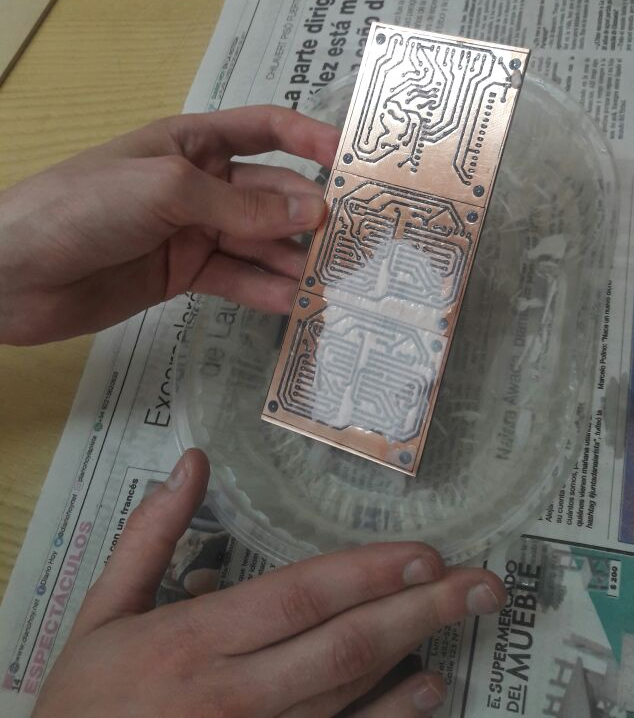
\includegraphics[width=0.6\linewidth]{imagenes/pcbeando/sacado-papel-1.png}
	\caption{Proceso de quitar el papel.}
	\label{fig:sacado-papel}
\end{figure}

\subsection{Reducción del Cobre}
Una vez quitado todo el papel debería quedar solo la tinta impregnada en el cobre (ver figura \ref{fig:pos-sacado-papel-1}). Si de alguna manera se salió la tinta, es posible corregir las imperfecciones con un marcador de esmalte, en la parte superior izquierda de la figura se puede notar que se requirio corregir el agujero del tornillo.

\begin{figure}[ht!]
	\centering
	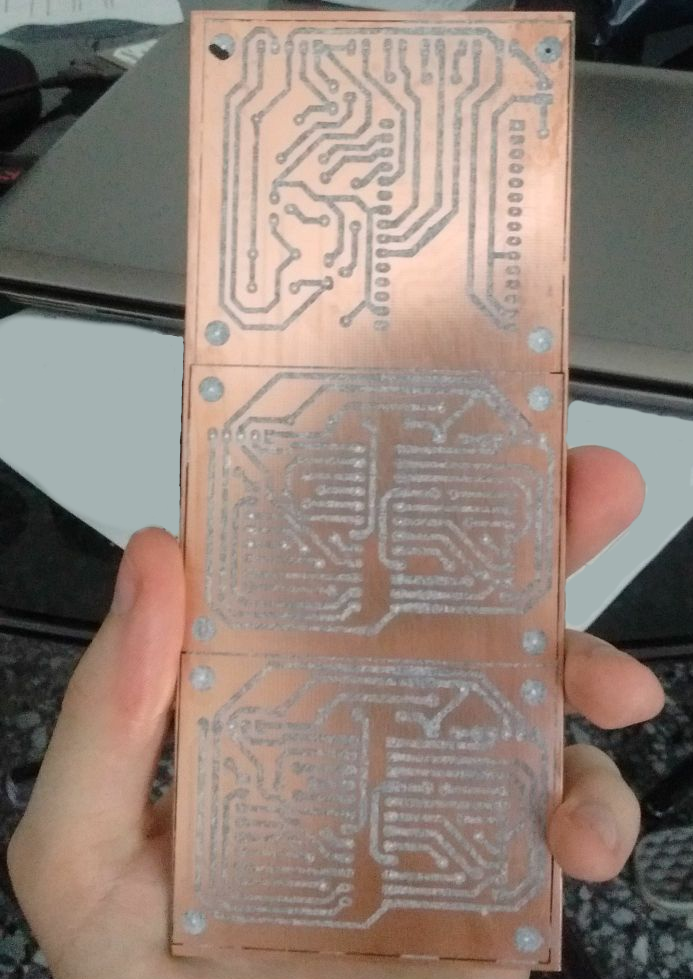
\includegraphics[width=0.5\linewidth]{imagenes/pcbeando/pos-sacado-pape-1.png}
	\caption{Pos sadcado papel.}
	\label{fig:pos-sacado-papel-1}
\end{figure}

{ \color{red} Contar que se opto por hacer GND toda una cara por lo tanto habia que pintar con esmalte la otra cara para que el cobre no lo comiera }
En la figura  \ref{fig:pos-sacado-papel-2} se puede ver el resultado luego de aplicar esmalte.

\begin{figure}[ht!]
	\centering
	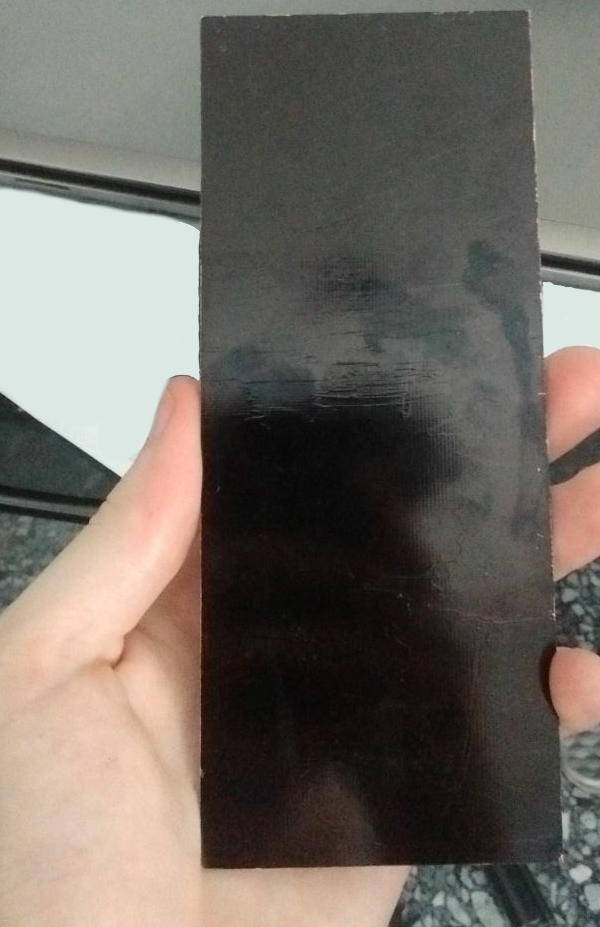
\includegraphics[width=0.5\linewidth]{imagenes/pcbeando/pos-sacado-papel-2.png}
	\caption{Pos sadcado papel 2.}
	\label{fig:pos-sacado-papel-2}
\end{figure}

Para reducir el cobre utilizar guantes de latex ya que el acido ferrico mancha.

{ \color{red} Contar el procedimiento del acido }

En la figura \ref{fig:pos-acido} se observa el resultado de ese paso.

\begin{figure}[ht!]
	\centering
	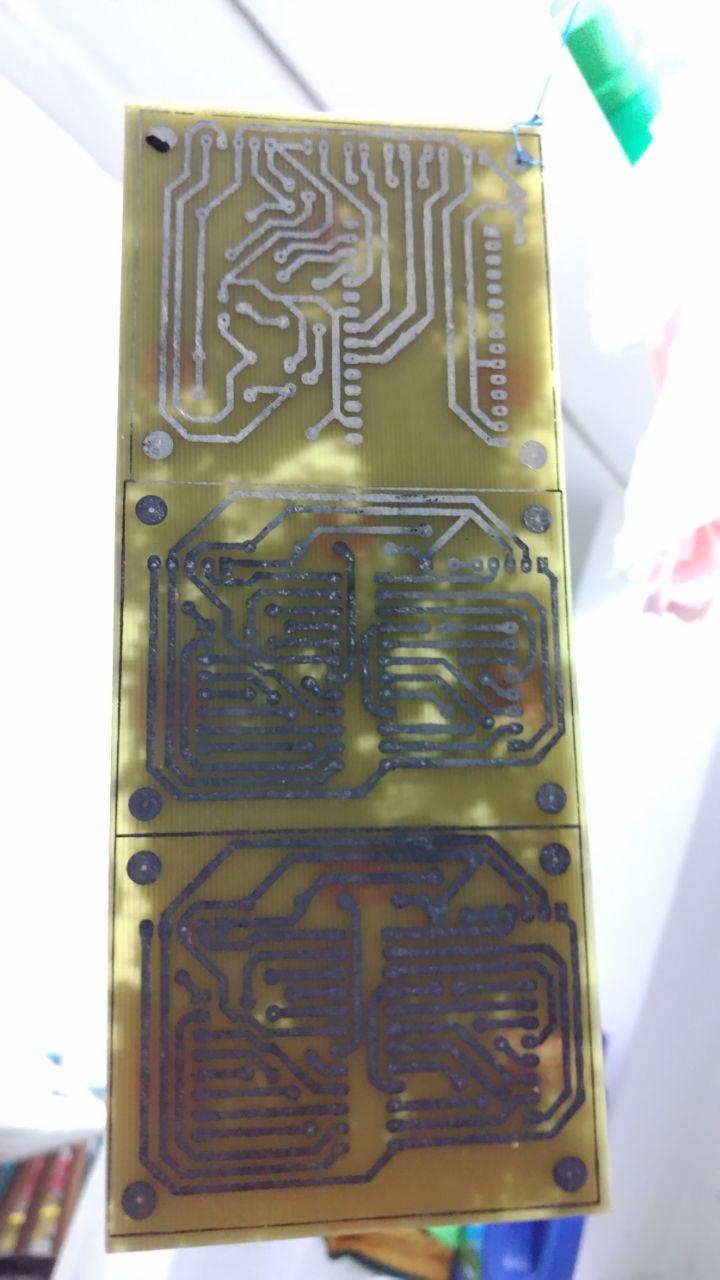
\includegraphics[width=0.5\linewidth]{imagenes/pcbeando/pos-acido.jpeg}
	\caption{Pos acido}
	\label{fig:pos-acido}
\end{figure}

\subsection{Perforado de Placas}
En este paso se requieren las mechas especificadas en el apéndice \ref{sec:materiales-para-hacer-cartel}.

\subsection{Montaje}


\section{Conclusiones}

Pudo comprobarse a través de este proyecto la viabilidad tanto en términos de hardware como de software del diseño planteado como implementación del cartel programable de LEDs. 
La totalidad del protocolo de comunicación pudo ser implementada de acuerdo a lo pautado en los objetivos iniciales, y en tiempo y forma respecto al cronograma propuesto. El desarrollo del hardware se vio demorado por falta de disposición de recursos, ya que algunos componentes no se encuentran disponibles en todas las tiendas de electrónica (Node MCU y MAX7219). Aún así pudo implementarse un prototipo del circuito maestro y dos prototipos de los circuitos esclavos, con las debidas interfaces para las conexiones externas e internas, tanto de datos como de alimentación, y cumpliendo los patrones de diseño recomendados por el personal técnico de la Facultad.

En términos de consumo, se comprobó que la potencia consumida por el circuito coincidía con la calculada mediante los datos indicados en la hoja de datos del MAX7219. Dicho consumo es relativamente bajo, por lo que no se lo considera un impedimento relevante a la hora de conseguir nuevas fuentes de alimentación para el sistema. 

Aunque no estaba planificado en el proyecto inicial el equipo también adaptó un cargador móvil en desuso para alimentar el circuito.

El presupuesto del proyecto cumplió con exactitud con lo planteado en la sección homónima del anexo.
% Explicar el grado de cumplimiento de objetivos planteados para el trabajo.
% Evaluar y destacar el cumplimiento y disvíos del cronograma de tareas presentados en el informe inicial
% Describir claramente la actividad de cada integrante del grupo, evaluar las horas invertidas por cada uno y calcular las horas de ingeniería total
% Analizar el presupuesto que se ha invertido y el presupuesto final del proyecto incluyendo las horas de ingeniería consumidas.
